\documentclass{suturo}

\begin{document}
    \maketitle{Motion}{29.12.2017}{}{1}{}{}{}{}

\makeatletter
\newcommand{\chapterauthor}[1]{%
  {\parindent0pt\vspace*{-27pt}%
  \linespread{0}\small\begin{flushright}von: #1\end{flushright}%
  \par\nobreak\vspace*{0pt}}
  \@afterheading%
}
\makeatother

\section{Node: main (motion\_suturo\_1718)}
\subsection{Architekturbild}
\chapterauthor{Roman Haak}
\begin{center} 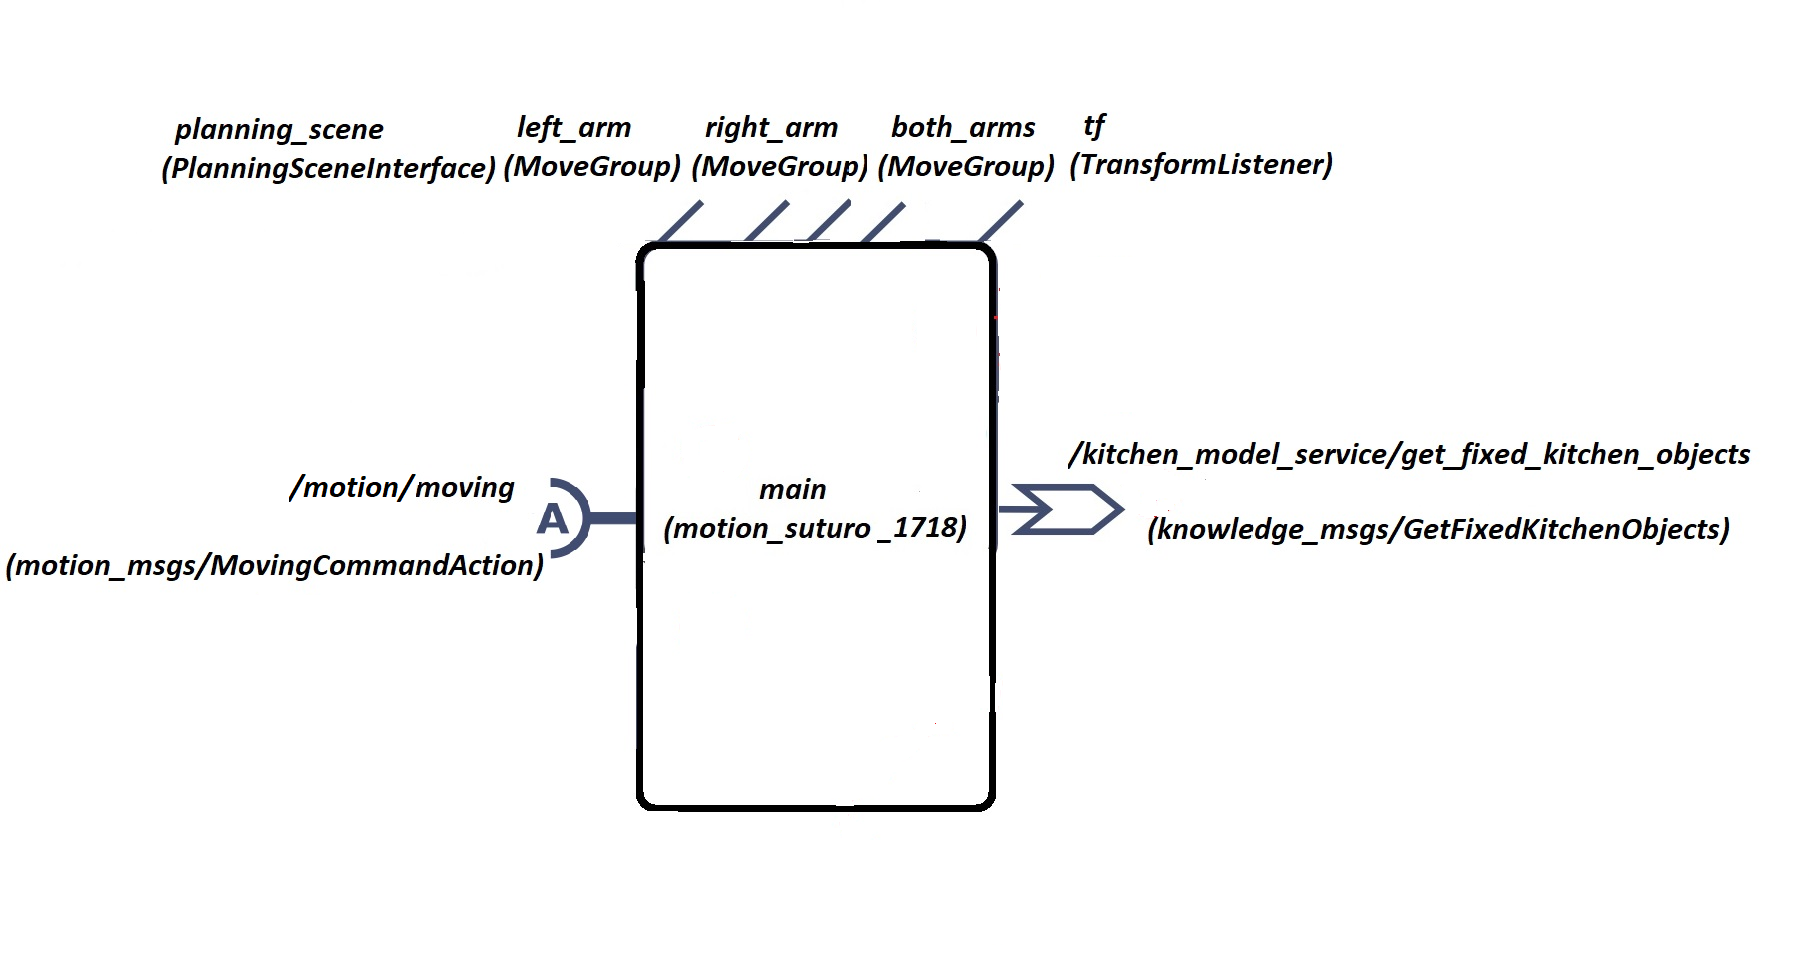
\includegraphics[width=0.8\textwidth]{img/Architekturbild.png} \end{center}

\subsection{API}
\subsubsection{Übersicht}
\chapterauthor{Roman Haak}
Dieser Teil des Systems ist für das Bewegen des PR2 in eine bestimmte Position, bzw. zu einem bestimmten Punkt hin verantwortlich.\\
Zum Ausführen von Bewegungen des PR2 benutzen wir das '\textit{MoveIt-Framework}'. Dieses Framework bietet dabei ein '\textit{MoveGroup-Interface}' an, mit dessen Hilfe es dem Benutzer möglich ist, mit einfachen Funktionsaufrufen Bewegungen auszuführen. Die dahinter steckenden Logiken und Umrechnungen, welche zum letztendlichen Bewegen des Armes nötig sind, werden dann von dem Framework umgesetzt, ohne dass der Benutzer sich darum kümmern muss.\\
Wie wir dieses Framework benutzen, wird im Folgenden vorgestellt.

\subsubsection{Klassenvariablen}
\chapterauthor{Roman Haak}
Im Folgenden werden kurz die wichtigsten Variablen der Klasse '\textit{main}' vorgestellt, um die Funktionsweise des \textit{MoveGrop-Interfaces} zu verdeutlichen:\\\\
\textit{\textbf{planning\_scene}} vom Typ \textit{\textbf{PlanningSceneInterface}}:\\
Über diese Variable ist es uns möglich die sogenannte '\textit{PlanningScene}' des PR2 zu befüllen. Über die \textit{PlanningScene} wird dem PR2 signalisiert, an welcher Stelle sich Objekte befinden, damit Kollisionen mit diesen Vermieden werden können. Wird von dem Benutzer versucht, über das \textit{MoveIt\_Framework} eine Bewegung auszuführen, prüft das Framework zunächst, ob diese Bewegung kollisionsfrei ausgeführt werden kann und bricht mit entsprechender Fehlermeldung ab, falls es in der \textit{PlanningScene} ein Objekt gibt, mit dem der PR2 kollidieren würde. \\
Die Objekte der PlanningScene sind in unserem Fall die Küchenobjekte der IAI-Küche und werden definiert durch einen '\textit{Box-Collider}' mit gewisser Höhe, Breite und Länge.\\\\
\textit{\textbf{both\_arms}}, \textit{\textbf{left\_arm}}, \textit{\textbf{right\_arm}} vom Typ \textit{\textbf{MoveGroupInterface}}:\\
Über Variablen des \textit{MoveGroupInterfaces} können Befehle zum Bewegen eines bestimmten Körperteils abgeschickt werden. Bei uns gibt es dabei drei Gruppen für linken, rechten und beide Arme.\\
So können wir den Endpunkt der jeweiligen kinematischen Kette zu einem bestimmten Punkt hinbewegen oder auch die Gelenkwinkel der Gelenke einer Gruppe einstellen. Das Berechnen einer Trajektorie übernimmt dabei das \textit{MoveIt-Framework}.\\
Es wird von dem \textit{MoveGroup}-Objekt eine entsprechende Rückmeldung in Form eines \textit{MoveItErrorCodes} über den Erfolg der Ausführung gegeben.\\\\
\textit{\textbf{tf}} vom Typ \textit{\textbf{TransformListener}}:\\
Mit Hilfe des \textit{TransformListeners} können Transformationen zwischen Koordinatensystemen zu einem bestimmten Zeitpunkt durchgeführt werden. Das ist in unserem Fall z.B. nötig, wenn der Arm zu einem bestimmten Punkt bewegt werden soll, der aber in einem anderen Koordinatensystem angegeben ist, als unser \textit{MoveGroup}-Objekt zum Planen verwendet.\\

\subsubsection{Serviceclient}
\chapterauthor{Roman Haak}
'\textit{/kitchen\_model\_service/get\_fixed\_kitchen\_objects}': \\
Dieser Service wird beim Initialisieren unseres Programms aufgerufen. Hierüber werden die Abmessungen der Objekte der IAI-Küche in die \textit{PlanningScene} geladen, damit der Roboter sich nur kollisionsfrei bewegt(siehe \textit{Kapitel 1.2.2}, Abschnitt zur '\textit{planning\_scene}').\\
Die Objekte sind dabei durch eine Höhe, Breite und Länge als \textit{Box-Collider} definiert.


\subsubsection{ActionServer}
\chapterauthor{Maximilian Bertram}
'\textit{/motion/moving}': \\
Vom Typ '\textit{motion\_msgs/MovingCommand}': \\
\begin{lstlisting}
#goal definition
geometry_msgs/PointStamped point_stamped
uint8 command
uint8 UNKNOWN=0
uint8 MOVE_STANDARD_POSE=1
uint8 MOVE_RIGHT_ARM=2
uint8 MOVE_LEFT_ARM=3
---
#result definition
bool successful
---
#feedback definition
#bool finished
\end{lstlisting}

%HIER NOCH DIE BESCHREIBUNG DES ACTIONSERVERS

\subsubsection{Programmablauf}
\chapterauthor{Maximilian Bertram}
%UNTERSCHIED LAUNCHFILE FÜR SIMULATION UND ECHTER ROBOTER -> LADEN DER KONFIGURATIONSDATEIEN - SIMULATION ODER ECHTER ROBOTER
%STARTEN DER NAVIGATIONSSACHEN -> AUCH HIER UNTERSCHIED SIMULATION UND ECHTER ROBOTER
%INITIALISIEREN DER KÜCHE, WARTEN AUF CALL DES ACTIONSERVERS, AUSFÜHREN (FALLS MÖGLICH), RÜCKMELDUNG AN ACTIONCLIENTS (IN SIMULATION UND ECHT GLEICH)
\subsubsection{Besonderheiten/Besondere Algorithmen}
\chapterauthor{Maximilian Bertram}
%ÜBERHAUPT VORHANDEN? PARSEN DER MOVEITERRORCODES? VISUALIZATION-MARKER? ORIENTATION DES GRIPPERS?


\end{document}
